%Revisado
\section{Fase 3: Expansão Espectral e Engenharia de Características (QP3)}
\label{sec:expansao_espectral}

Nesta fase, avaliou-se a Questão de Pesquisa QP3, que propunha que a expansão digital do espectro (15 canais gerados via filtros de Gabor) auxiliaria as redes a extrair texturas mais ricas da fibra. O experimento consistiu no treinamento paralelo de modelos nos conjuntos de dados \textbf{AB}, \textbf{AM} e \textbf{BR}, comparando-os aos seus equivalentes RGB sob as mesmas condições de iluminação.

O contraste de desempenho, ilustrado na Figura \ref{fig:h3_spectral}, revela uma queda drástica e generalizada no MCC para todas as versões com expansão espectral. Este fenômeno permite rejeitar a hipótese nula $H_{0,3}$, respondendo negativamente à QP3 e indicando que para modelos de \textit{Deep Learning} modernos, a inserção de \textit{features} artesanais ruidosas ou redundantes atua como um mecanismo de confusão no aprendizado \textit{end-to-end}.

\begin{figure}[h!]
  \centering
  \caption{Falha da Expansão Espectral (QP3): O contraste entre o RGB puro (3ch) e os 15-canais Gabor mostra a severa degradação da performance em todos os cenários de luz.}
  \label{fig:h3_spectral}
  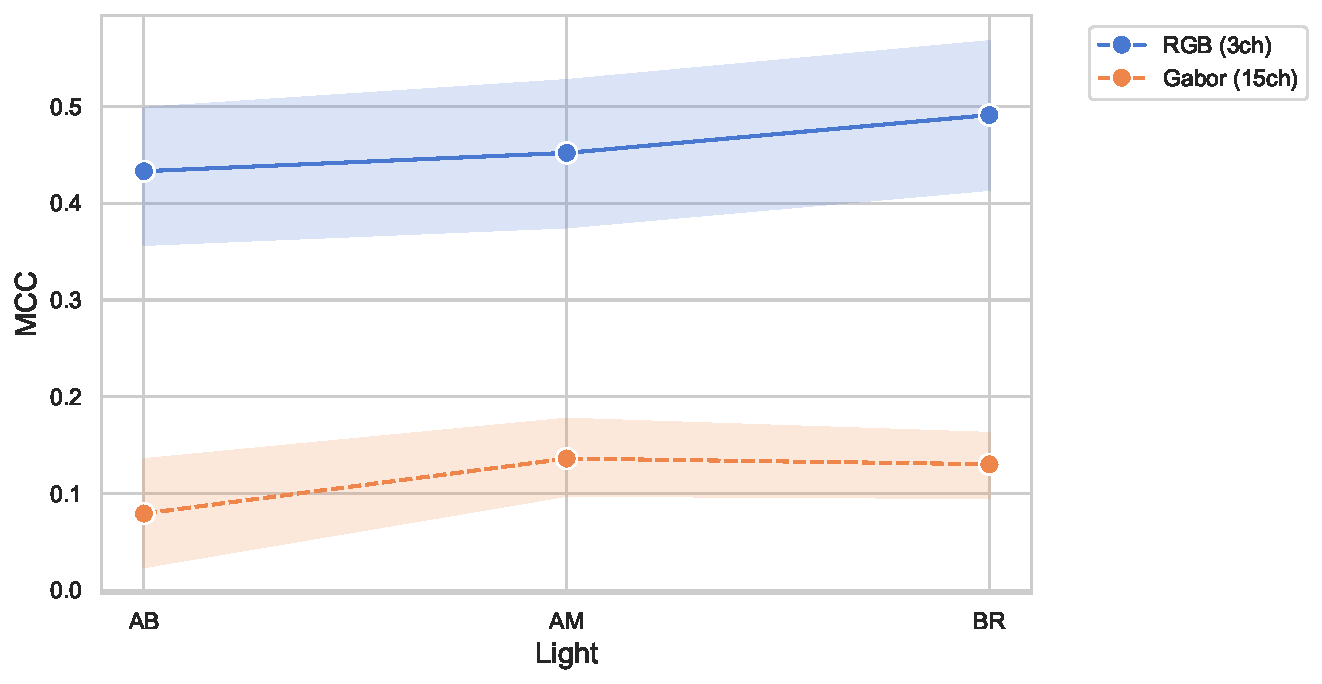
\includegraphics[width=0.8\textwidth]{images/h3_spectral_impact.pdf}
  \legend{Fonte: Do autor (2026).}
\end{figure}

Para validar se esta queda de performance foi estatisticamente relevante, aplicou-se o \textbf{teste de McNemar} (binomial exato, sem a correção de continuidade de Yates) pareado por arquitetura no cenário de melhor iluminação (Luz Branca BR). O teste compara, para cada arquitetura, os \textit{patches} discordantes entre o classificador treinado sobre RGB puro e o seu equivalente treinado sobre o tensor expandido de 15 canais Gabor: $b$ é a contagem de \textit{patches} que o modelo RGB acertou e o modelo Gabor errou, e $c$ é a contagem inversa (Gabor acertou, RGB errou). A hipótese nula $H_{0,3}$ (Seção \ref{sec:desenho_experimental}) postula que as duas variantes cometem a mesma proporção de erros, isto é, $b = c$ na população. Conforme apresentado na Tabela \ref{tab:mcnemar_gabor}, a degradação foi severa e sistemática para todos os modelos, com $c \gg b$ em todos os pares --- a \textbf{DenseNet}, por exemplo, sofreu uma redução de MCC de $0,6461$ para $0,1577$, enquanto a \textbf{ConvNext} caiu de $0,6153$ para $0,1282$.

\begin{table}[!h]
    \centering
    \begin{threeparttable}
    \caption{Teste de McNemar comparando RGB (V10) e Gabor (V12) sob Luz Branca.}
    \label{tab:mcnemar_gabor}
    \begin{tabular}{lrrl}
\toprule
Modelo & MCC (RGB) & MCC (Gabor) & p-value \\
\midrule
RESNET & 0.4501 & 0.0869 & 9.80e-85 \\
DENSENET & 0.6461 & 0.1577 & 2.40e-136 \\
EFFICIENTNET & 0.5915 & 0.2280 & 8.05e-66 \\
CONVNEXT & 0.6153 & 0.1282 & 5.63e-116 \\
VGG & 0.4910 & 0.1548 & 4.88e-69 \\
SWIN & 0.4143 & 0.1273 & 1.43e-54 \\
VIT & 0.4328 & 0.1158 & 3.62e-60 \\
INCEPTION & 0.2882 & 0.0421 & 4.62e-51 \\
\bottomrule
\end{tabular}

    \begin{tablenotes}
            \small 
            \item[] Fonte: Do autor (2026).
        \end{tablenotes}
        \end{threeparttable}
\end{table}

Os valores $b$, $c$ e os $p$-values reportados na Tabela \ref{tab:mcnemar_gabor} permitem rejeitar $H_{0,3}$ para os oito pares comparados, confirmando que a diferença de performance não é fruto do acaso, mas sim de uma incapacidade sistemática dos modelos em lidar com a dimensionalidade ruidosa dos filtros de Gabor. Conclui-se que, para este domínio, a simplicidade do sinal bruto de entrada é superior à complexidade algorítmica de pré-processamento clássico, validando a preferência por aprendizado profundo puramente orientado a dados.
